\input ../SlidePreamble
\input ../preamble


\begin{document}

{\Huge

  \centerline{\bf TTIC 31230, Fundamentals of Deep Learning}
  \bigskip
  \centerline{David McAllester, Autumn 2022}
  \vfill
  \vfil
  \centerline{Diffusion Model Basics}
  \vfill
  \vfill

\slidetwo{Denoising Diffusion Probabilistic Models (DDPM)}{Ho, Jain and Abbeel, June 2020}

\centerline{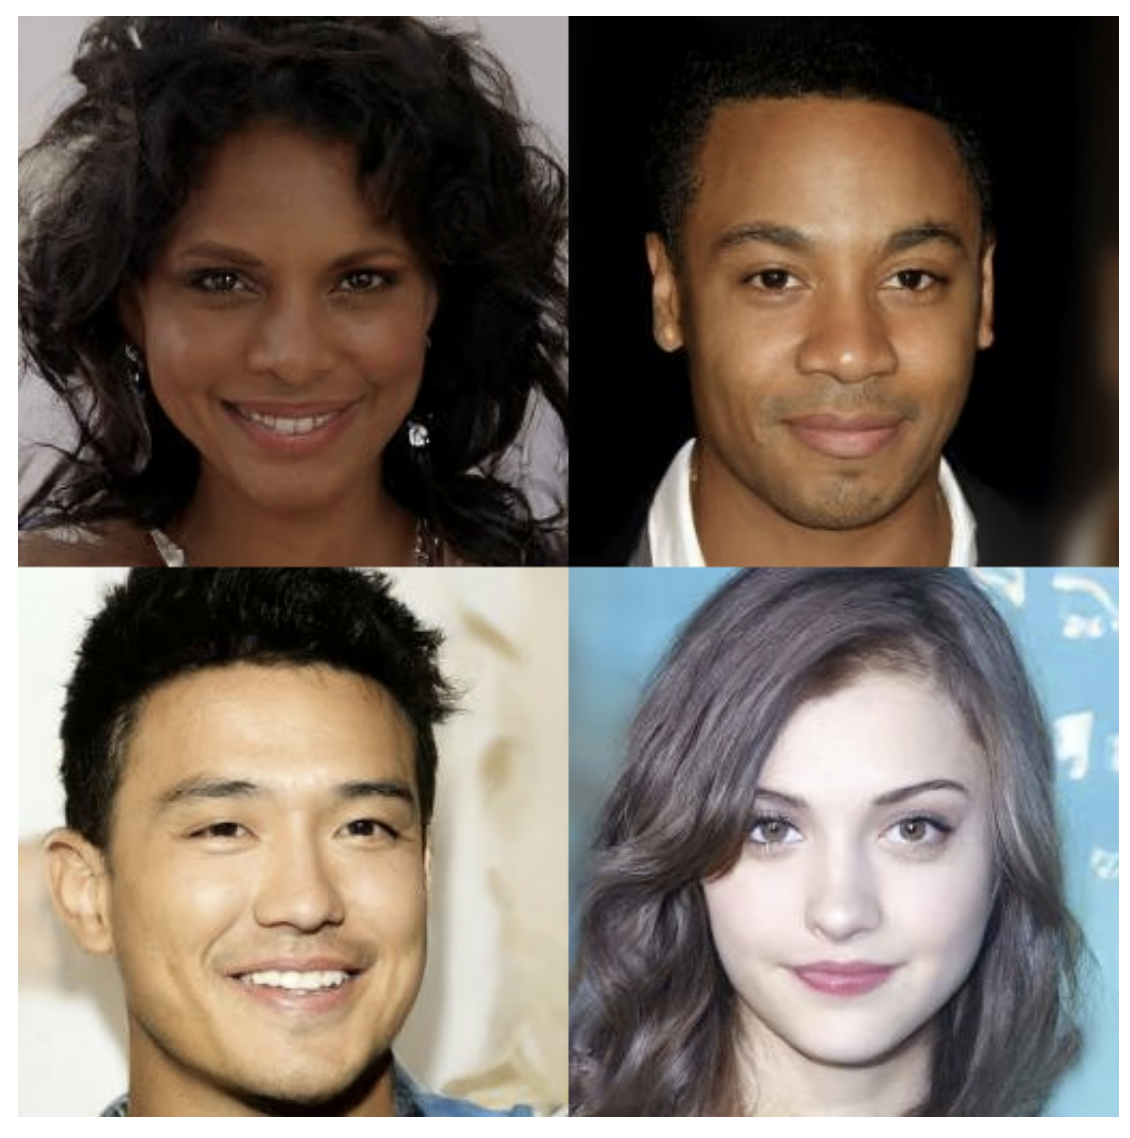
\includegraphics[width = 4in]{\images/DiffCeleb}}


\slide{Markovian VAEs}

A diffusion model (DDPM) is a Markovian VAE.

\vfill
We model $y$ with a latent variable $z =(z_0,z_1,\dots,z_{L})$.

\vfill
The encoder is defined by $z_0 = y$ and $P_\enc(z_\ell|z_{\ell-1})$.

\vfill
The prior is defined by $P_\pri(z_L)$ and $P_{\pri}(z_{\ell-1}|z_{\ell})$ and subsumes the decoder as $P_\pri(z_0|z_1)$.

\slide{Markovian VAEs}

We model $y$ with a latent variable $z =(z_0,z_1,\dots,z_{L})$.

\vfill
The encoder is defined by $z_0 = y$ and $P_\enc(z_\ell|z_{\ell-1})$.

\vfill
The prior is defined by $P_\pri(z_L)$ and $P_{\pri}(z_{\ell-1}|z_{\ell})$.

\vfill
We can generate $y$ by sampling from the prior.

\slide{Denoising Diffusion Probabilistic Models (DDPM)}

We model $y$ with a latent variable $z =(z_0,z_1,\dots,z_{L})$ with $z_0 = y$.

\vfill
In a DDPM we have that $z_\ell$ is the result of adding noise to the given image $y$.

\centerline{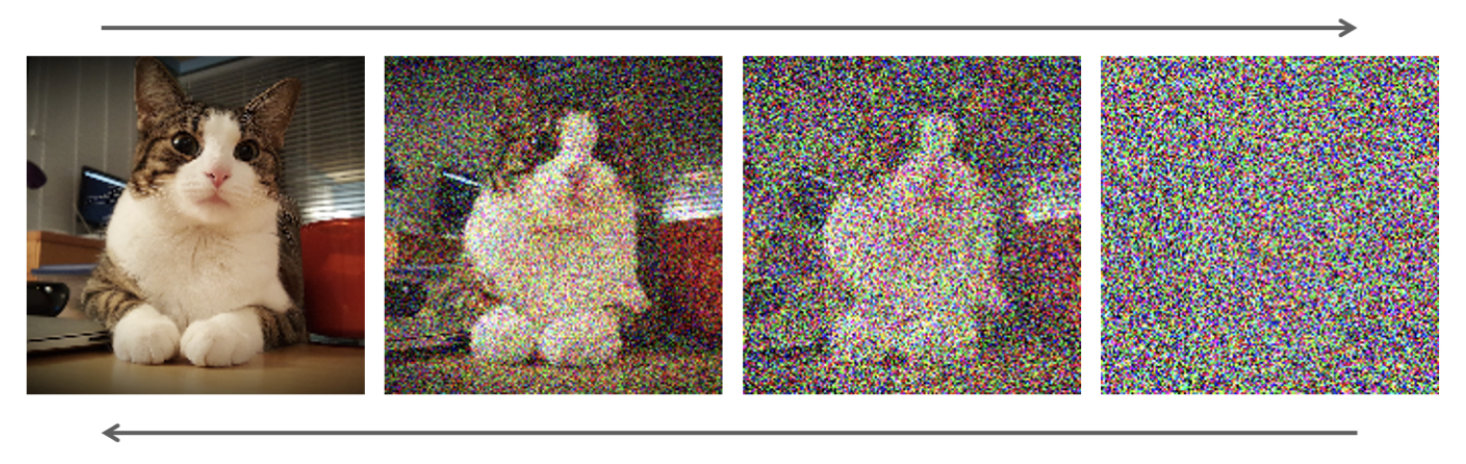
\includegraphics[width = 7in]{\images/DiffSequence}}


\slide{DDPM SDE}

The DDPM stochastic differential equation (SDE) provides the formal motivation for DDPM models.

\vfill
{\bf For the DDPM SDE one can show analytically that the true reverse process probabilities  $P(z_{\ell-1}|z_\ell)$ (as defined by the forward process)
are Gaussians with a known variance.}

\vfill
This implies that in the SDE limit we can model any population {\bf exactly} by a model in which $P(z_{\ell-1}|z_\ell)$ is taken to be Gaussian.

\slide{DDPM SDE}

To formulate the DDPM SDE we will use the same $\sigma$ at all levels.

$$\mathrm{for}\;\ell \geq 1\;\;\;\;z_\ell = \sqrt{1-\sigma^2}\;z_{\ell-1} + \sigma \epsilon\;\;\;\;\epsilon \sim {\cal N}(0,I)$$

\vfill
This is designed so that if $z_{\ell-1}$ has unit variance in each dimension then $z_{\ell}$ also has unit variance in each dimension.

\vfill
$z_0 = y$ is scaled so that each coordinate is in the interval $[0,1]$ so that all $z_\ell$ have approximately unit variance.

\slide{DDPM SDE}

$$\mathrm{for}\;\ell \geq 1\;\;\;\;z_\ell = \sqrt{1-\sigma^2}\;z_{\ell-1} + \sigma \epsilon\;\;\;\;\epsilon \sim {\cal N}(0,I)$$

\vfill
Unit Variance is desired because in implementations the same prior network is used
for all levels and it is then important that $z_\ell$ has the same scale and variance for all $\ell$.

\slide{DDPM SDE}

Because a sum of independent Gaussians is also a Gaussian, we can sample $z_{\ell}$ directly from $z_0$.

$$\mathrm{define}\;\;\;\alpha = \sqrt{1-\sigma^2}$$

\vfill
$$z_{\ell} = \alpha^\ell z_0 + \sqrt{1-\alpha^{2\ell}} \;\epsilon\;\;\;\epsilon \sim {\cal N}(0,I)$$

\vfill
The variance of the noise term follows from the fact that $z_{\ell}$ has unit variance in each dimention when $z_{\ell-1}$ does.

\slide{DDPM SDE}

We select the endpoint $L$ such that $z_L$ is essentially all noise.

$$z_{L} = \alpha^L z_0 + \sqrt{1-\alpha^{2L}} \;\epsilon\;\;\;\epsilon \sim {\cal N}(0,I)$$

\vfill
For some limit $\delta$ we select $L$ to be the least integer satisfying

\begin{equation}
\label{eq:L}
\alpha^L = \sqrt{1-\sigma^2}^L < \delta
\end{equation}

\vfill
The stochastic differential equation is defined by simultaneously taking $\sigma \rightarrow 0$ and $L \rightarrow \infty$ while satisfying (\ref{eq:L}).

\slide{DDPM SDE}

\begin{eqnarray*}
z_t& = & e^{-t}z_0 + \sqrt{1 - e^{-2t}}\;\epsilon_1 \\
\\
\Delta z & = & - z_t \Delta t + \sqrt{2\Delta t} \epsilon_2
\end{eqnarray*}

\vfill
A first observation is that for infinitisimal $\Delta t$ we have that $\Delta t$  is infinitesmal compared to $\sqrt{2\Delta t}$.  {\bf Hence the
distribution $P(\Delta z|z_{t},\Delta t)$ is Gaussian with variance $\sigma = \sqrt{2\Delta t}$ and with mean infinitesimal with respect to the variance.}

\slide{DDPM SDE}

\begin{eqnarray*}
z_\ell& = & \sqrt{1 - \sigma^2}\;z_{\ell-1} + \sigma\;\epsilon \\
\end{eqnarray*}

As we take $\sigma \rightarrow  0$ we can rewrite $\sqrt{1-\sigma^2}$ using the first order Taylor expansion of the square root function.

\begin{eqnarray*}
z_\ell & = &  \left(1 - \frac{1}{2}\sigma^2\right)\;z_{\ell-1} + \sigma\;\epsilon \\
\\
\Delta z & = &  - \frac{1}{2}\sigma^2\;z_{\ell-1} + \sigma\;\epsilon
\end{eqnarray*}

\slide{DDPM SDE}

$$\Delta z  =   - \frac{1}{2}\sigma^2\;z_{\ell-1} + \sigma\;\epsilon$$

\vfill
Here we are taking $\sigma \rightarrow 0$ which means that the second order term $(1/2)\sigma^2 z_\ell$ is infintesimal compared to the noise term
$\sigma \epsilon$.  This is the hallmark of a stochastic differential equation.

\vfill
Here $\Delta z$ is distributed as a Gaussian with variance $\sigma$ and an infinitesimal mean (relative to its variance).  The mean is infinitesimal compared to the variance,
the mean accumulutes over the (very large) sequence $z_0,\ldots, z_L$.

\slide{Rewriting the ELBO}
We will derive the structure of the prior by optimizing the ELBO loss.

\vfill
The following is a standard reformulation of the ELBO loss that is valid for all Markovian VAEs.

{\huge
\begin{eqnarray*}
H(z_0) & \leq & E_{y,z}\; -\ln \frac{p_\pri(z_0,\ldots,z_L)}{p_\enc(z_1,\ldots,z_L|z_0)}
\\
\\
\\
& = & E_{y,z} -\ln p_\pri(z_L) - \sum_{\ell \geq 1} \frac{\ln p_\pri(z_{\ell-1}|z_\ell)}{\ln p_\enc(z_\ell|z_{\ell-1})}
\end{eqnarray*}
}


\slide{Rewriting the ELBO}

{\huge
\begin{eqnarray*}
H(z_0) & \leq & E_{y,z} -\ln p_\pri(z_L) - \sum_{1 \leq \ell \leq L } \ln \frac{p_\pri(z_{\ell-1}|z_\ell)}{p_\enc(z_\ell|z_{\ell-1})} \\
\\
& = & E_{y,z} -\ln p_\pri(z_L) - \sum_{1 \leq \ell\leq L } \ln \frac{p_\pri(z_{\ell-1}|z_\ell)}{p_\enc(z_\ell|z_{\ell-1},z_0)} \\
\\
& = & E_{y,z} -\ln p_\pri(z_L) - \sum_{1 \leq \ell\leq L } \ln \frac{p_\pri(z_{\ell-1}|z_\ell)p(z_{\ell-1}|z_0)}{p_\enc(z_\ell,z_{\ell-1}|z_0)} \\
\\
& = & E_{y,z} -\ln p_\pri(z_L) - \sum_{1 \leq \ell\leq L } \ln \frac{p_\pri(z_{\ell-1}|z_\ell)p_\enc(z_{\ell-1}|z_0)}{p_\enc(z_{\ell-1}|z_\ell,z_0)p_\enc(z_\ell|z_0)}
\end{eqnarray*}
}

\slide{Rewriting the ELBO}

{\huge
\begin{eqnarray*}
H(z_0) & \leq & E_{y,z} -\ln p_\pri(z_L) - \sum_{1 \leq \ell\leq L } \ln \frac{p_\pri(z_{\ell-1}|z_\ell)}{p_\enc(z_{\ell-1}|z_\ell,z_0)}
- \ln \frac{p_\pri(z_{\ell-1}|z_0)}{p_\enc(z_\ell|z_0)} \\
\\
& = & E_{y,z} -\ln \frac{p_\pri(z_L)}{p_\enc(z_L|z_0)} - \sum_{{\color{red} 2} \leq \ell \leq L} \ln \frac{p_\pri(z_{\ell-1}|z_\ell)}{p_\enc(z_{\ell-1}|z_\ell,z_0)} - \ln p_\pri(z_0|z_1) \\
\\
\\
& = & {\color{red} E_{y,z} \left\{\begin{array}{l}KL(p_\enc(z_L|z_0),p_\pri(z_L)) \\
\\
+ \sum_{2 \leq \ell \leq L} KL(p_\enc(z_{\ell-1}|z_\ell,z_0),p_\pri(z_{\ell-1}|z_\ell)) \\
\\
- \ln p_\pri(z_0|z_1) \end{array} \right.}
\end{eqnarray*}
}

\slide{Using The Gaussian Model}

The ELBO loss is optimized by

$$\pri^*(z_{\ell-1}|z_\ell)  = \argmin_\pri\;E_{y,z}\;\ln  \frac{\;p_\enc(z_{\ell-1}|z_\ell,y)}{p_\pri(z_{\ell-1}|z_\ell)}$$

In the DDPM SDE both distributions are Gaussians with variance $\sigma$.  The KL divergence then becomes.

$$\pri^* = \argmin_\pri \;\sum_\ell \;E_{y,z}\;\frac{||\mu_\pri(z_{\ell-1}|z_\ell) - \mu_\enc(z_{\ell-1}|z_\ell,y)||^2}{2\sigma^2}$$

\slide{Setting the Variance to $\sigma$ in the prior.}

$$\pri^* = \argmin_\pri \;\sum_\ell \;E_{y,z}\;\frac{||\mu_\pri(z_{\ell-1}|z_\ell) - \mu_\enc(z_{\ell-1}|z_\ell,y)||^2}{2\sigma^2}$$

$$\pri^* = \argmin_{\pri}\;\;\sum_\ell\;E_{z_0,\ell,z_{\ell-1},z_\ell} \;\;\frac{||\mu_\pri(\ell,z_\ell) - z_{\ell-1}||^2}{2\sigma^2}$$

\vfill
The natural thing now is to train $\mu_\pri(\ell,z_\ell)$ to predict $z_{\ell-1}$.

\slide{Reducing the Prior's Dependence on $\ell$.}

We have already reduced the prior's dependence on $\ell$ by making $z_\ell$ have unit variance for all $\ell$.

\vfill
But additional dependence on $\ell$ can still be removed.

\vfill
First we solve for $z_{\ell-1}$ in terms of $z_\ell$ and $\epsilon$.

{\huge
$$z_\ell = \sqrt{1-\sigma^2_\ell}\;z_{\ell-1} + \sigma \epsilon\;\;\;\;\epsilon \sim {\cal N}(0,I)$$

\vfill
$$z_{\ell-1} = \frac{1}{\sqrt{1-\sigma^2}}(z_\ell - \sigma \epsilon)$$

\vfill
$$\mu_\pri(\ell,z_\ell) = \frac{1}{\sqrt{1-\sigma^2}}\left(z_\ell - \sigma\; \epsilon_\pri(\ell,z_\ell)\right)$$
}

\vfill
Here $\epsilon_\pri(\ell,z_\ell)$ is a trained network whose target value has the same behavior at all levels of $\ell$.

\slide{An $\epsilon$-Prior}

$$\mu_\pri(\ell,z_\ell) = \frac{1}{\sqrt{1-\sigma^2}}\left(z_\ell - \sigma\; \epsilon_\pri(\ell,z_\ell)\right)$$

\vfill
However, SGD on the loss $\left|\left|z_{\ell-1} - \mu_\pri(\ell,z_\ell)\right|\right|^2$ now scales the SGD gradients on $\Phi$ differently for different $\ell$.

\vfill
We effectively have different learning rates for different $\ell$.

\slide{Training the $\epsilon$-Prior}

To make the scale of the SGD gradients independent of $\ell$ we use the following loss.

\vfill
$$\Phi^* = \argmin_{\Phi}
\left\{\begin{array}{l}\;E_{z_0,\ell,z_{\ell-1},\epsilon \sim {\cal N}(0,I)}\; \\
\\
~\;\;\;\;\left|\left|\epsilon - \epsilon_\pri\left(\ell,z_\ell(z_{\ell-1}),\ell)\right)\right|\right|^2
\end{array}\right.$$

\vfill
We now repeatedly sample $z_0$, $\ell$, $z_{\ell-1}$ and $\epsilon$ and do gradient updates on $\Phi$.

\slide{$\epsilon$-Prior Architecture}

The $\epsilon$-decoder is a U-Net.

\centerline{\includegraphics[width = 8in]{\images/U-NET}}

\slide{Generating Faces}

\centerline{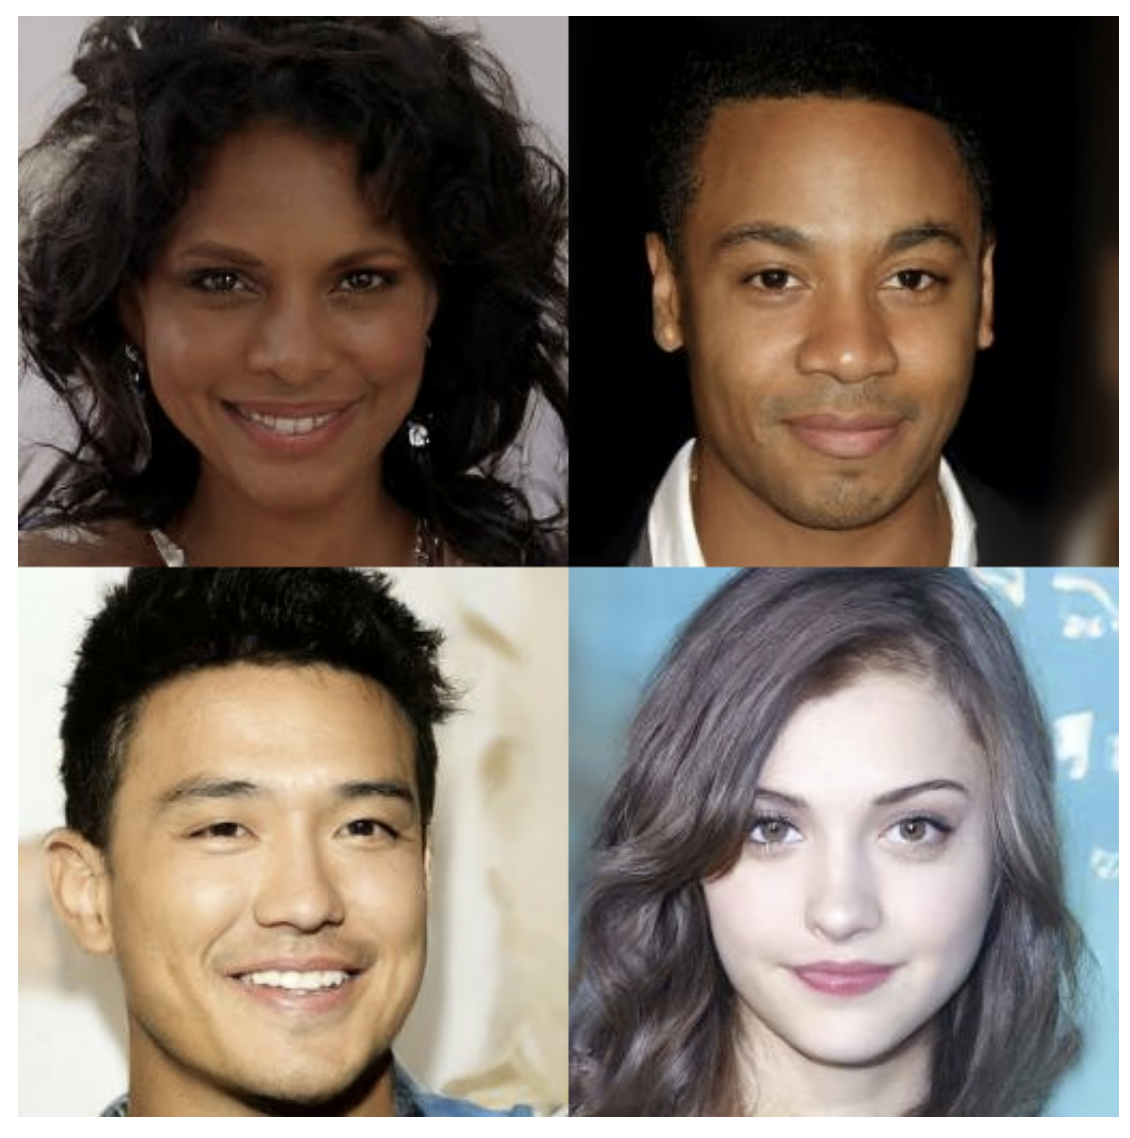
\includegraphics[width = 3.5in]{\images/DiffCeleb}}

\vfill
But this is ``mearly'' a face generator. DALLE and DALLE-2 do text-conditioned image generation.  Also, here we are using $L = 1000$.
\slide{END}
}
\end{document}

